\documentclass[10pt]{article}
\usepackage[english]{babel}
\usepackage{../../../../lib/tex/naproche}
\usepackage{amssymb}
\usepackage{mathtools} % for \coloneq

\usepackage{stex-highlighting}
\providebool{emph} % "\newbool{emph}" does not work...
\setbool{emph}{false}
\colorlet{emphcolor}{violet}
\let\oldemph\emph
\renewcommand\emph[1]{\setbool{emph}{true}\ifbool{forthel}{\textcolor{emphcolor}{\itshape#1}}{\oldemph{#1}}\setbool{emph}{false}}
\renewcommand{\varemph}[1]{\ifbool{emph}{\textcolor{emphcolor}{#1}}{\textcolor{black}{#1}}}

\usepackage[right=6cm,left=3cm,bottom=3cm,marginparwidth=5cm]{geometry}

\usepackage{fancyhdr}
\renewcommand{\sectionmark}[1]{\markboth{#1}{}} 
\def\libarchive{}
\pagestyle{fancy}
\fancyhead[L]{\libarchive}
\fancyhead[C]{\nouppercase\leftmark}  % section title
\fancyhead[R]{\thepage}               % page number
\fancyfoot[C]{}                       % No page number in footer

\usepackage[nobottomtitles]{titlesec}
\titlespacing*{\section}{0pt}{30pt}{0pt}
\titlespacing*{\subsection}{0pt}{30pt}{0pt}
\titlespacing*{\subsubsection}{0pt}{30pt}{0pt}

\documentclass[12pt,oneside]{book}

\usepackage[foundations]{../../lib/tex/naproche}
\usepackage{../../lib/tex/libraries}
\usepackage{graphicx}
\usepackage{float}
\usepackage{caption}
\usepackage{footnote}

\makesavenoteenv{tabular} % Make footnotes work in tabular environments


\title{Foundations of Mathematics}
\author{Marcel Schütz}
\date{2022}

\begin{document}
  \maketitle

  \tableofcontents

  \begin{figure}[H]
    \centering
    \fbox{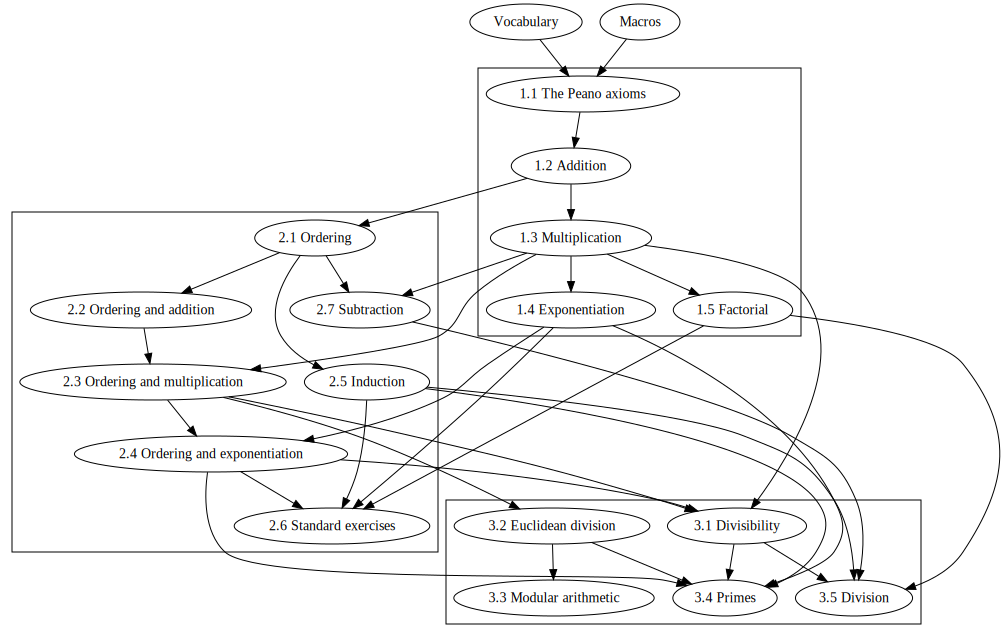
\includegraphics[width=0.9\linewidth]{./dependency-graph/graph.png}}
    \caption*{Interdependencies of the chapters}
  \end{figure}


  \section*{Introduction}

  This is a library providing a foundation of mathematics based on a
  Kelley-Morse like class theory with urelements.
  It introduces common operations on classes like unions or intersections
  (\cref{chapter:classes}) together with detailed proofs of their algebraic
  properties (\cref{chapter:computation-laws-for-classes}), the symmetric
  difference of two classes (\cref{chapter:symmetric-difference}) and the
  notions of ordered pairs and Cartesian products
  (\cref{chapter:pairs-and-products}) as well as proofs of the algebraic
  properties of the latter (\cref{chapter:computation-laws-for-products}).
  Moreover, it provides common operations on maps (\cref{chapter:maps}), various
  properties of images and preimages (\cref{chapter:image-and-preimage}) and the
  notions of injectivity, surjectivity, bijectivity
  (\cref{chapter:injections-surjections-bijections}) and invertibility of maps
  (\cref{chapter:invertible-maps}).
  The library provides an axiom system characterizing sets (\cref{chapter:sets})
  and, furthermore, it covers the notions of binary relations
  (\cref{chapter:binary-relations}), fixed-points of subset preserving maps
  (\cref{chapter:fixed-points}), including and equinumerosity
  (\cref{chapter:equinumerosity}).

  As two famous results it includes the Knaster-Tarski fixed point theorem
  (\cref{FOUNDATIONS_12_8420450166112256}) and the Cantor-Schröder-Bernstein
  theorem (\cref{FOUNDATIONS_13_1913663275401216}).

  \paragraph*{Usage.}
  At the very beginning of each chapter you can find the name of its source
  file, e.g. \path{foundations/sections/01_classes.ftl.tex} for
  \cref{chapter:classes}. This filename can be used to import the chapter via
  \Naproche's \texttt{readtex} instruction to another ForTheL text, e.g.:
  \begin{center}
    \verb`[readtex \path{foundations/sections/01_classes.ftl.tex}]`
  \end{center}

  \paragraph*{Checking times.}
  The checking times for each of the chapters may vary from computer to
  computer, but on mid-range hardware they are likely to be similar to those
  given in table below:

  \begin{center}
    \begin{tabular}{c|c|c}

      & \multicolumn{2}{c}{\textbf{Checking time}}
      \\
      \textbf{Chapter}
      & \textbf{without dependencies}     & \textbf{with dependencies}
      \\ \hline
      \ref{chapter:classes}
      & 00:04 min                         & 00:04 min
      \\
      \ref{chapter:computation-laws-for-classes}
      & 00:12 min                         & 00:16 min
      \\
      \ref{chapter:symmetric-difference}
      & 00:32 min                         & 00:48 min
      \\
      \ref{chapter:pairs-and-products}
      & 00:08 min                         & 00:12 min
      \\
      \ref{chapter:computation-laws-for-products}
      & 01:36 min                         & 01:56 min
      \\
      \ref{chapter:maps}
      & 01:13 min                         & 01:25 min
      \\
      \ref{chapter:image-and-preimage}
      & 01:28 min                         & 02:53 min
      \\
      \ref{chapter:injections-surjections-bijections}
      & 00:38 min                         & 02:03 min
      \\
      \ref{chapter:invertible-maps}
      & 02:20 min                         & 04:23 min
      \\
      \ref{chapter:sets}
      & 02:17 min                         & 06:40 min
      \\
      \ref{chapter:binary-relations}
      & 00:14 min                         & 06:54 min
      \\
      \ref{chapter:fixed-points}
      & 00:33 min                         & 07:13 min
      \\
      \ref{chapter:equinumerosity}
      & 01:48 min                         & 09:01 min
    \end{tabular}
  \end{center}


  \subfile{sections/01_classes.ftl.tex}
  \subfile{sections/02_computation-laws-for-classes.ftl.tex}
  \subfile{sections/03_symmetric-difference.ftl.tex}
  \subfile{sections/04_pairs-and-products.ftl.tex}
  \subfile{sections/05_computation-laws-for-products.ftl.tex}
  \subfile{sections/06_maps.ftl.tex}
  \subfile{sections/07_image-and-preimage.ftl.tex}
  \subfile{sections/08_injections-surjections-bijections.ftl.tex}
  \subfile{sections/09_invertible-maps.ftl.tex}
  \subfile{sections/10_sets.ftl.tex}
  \subfile{sections/11_binary-relations.ftl.tex}
  \subfile{sections/12_fixed-points.ftl.tex}
  \subfile{sections/13_equinumerosity.ftl.tex}
\end{document}

\begin{document}
  \begin{imports}
    \begin{forthel}
      %[prove off][check off]

      [readtex \path{libraries/source/foundations/10_sets.ftl.tex}]

      %[prove on][check on]
    \end{forthel}
  \end{imports}


  \section{Binary Relations}

  \begin{forthel}
    \begin{definition}\printlabel{FOUNDATIONS_11_6429308924985344}
      A binary relation is a class $R$ such that every element of $R$ is a pair.
    \end{definition}
  \end{forthel}

  \begin{forthel}
    \begin{definition}\printlabel{FOUNDATIONS_11_1126092393938944}
      Let $R$ be a binary relation and $A$ be a class.
      $R$ is reflexive on $A$ iff for all $a \in A$ we have $(a,a) \in R$.
    \end{definition}
  \end{forthel}

  \begin{forthel}
    \begin{definition}\printlabel{FOUNDATIONS_11_365656446861312}
      Let $R$ be a binary relation and $A$ be a class.
      $R$ is irreflexive on $A$ iff for no $a \in A$ we have $(a,a) \in R$.
    \end{definition}
  \end{forthel}

  \begin{forthel}
    \begin{definition}\printlabel{FOUNDATIONS_11_2056300137545728}
      Let $R$ be a binary relation and $A$ be a class.
      $R$ is symmetric on $A$ iff for all $a, b \in A$ if $(a,b) \in R$ then
      $(b,a) \in R$.
    \end{definition}
  \end{forthel}

  \begin{forthel}
    \begin{definition}\printlabel{FOUNDATIONS_11_8301693043212288}
      Let $R$ be a binary relation and $A$ be a class.
      $R$ is antisymmetric on $A$ iff for all distinct $a, b \in A$ we have
      $(a,b) \notin R$ or $(b,a) \notin R$.
    \end{definition}
  \end{forthel}

  \begin{forthel}
    \begin{definition}\printlabel{FOUNDATIONS_11_6895428727472128}
      Let $R$ be a binary relation and $A$ be a class.
      $R$ is asymmetric on $A$ iff for all $a, b \in A$ if $(a,b) \in R$ then
      $(b,a) \notin R$.
    \end{definition}
  \end{forthel}

  \begin{forthel}
    \begin{definition}\printlabel{FOUNDATIONS_11_5377309666181120}
      Let $R$ be a binary relation and $A$ be a class.
      $R$ is transitive on $A$ iff for all $a, b, c \in A$ if $(a,b) \in R$ and
      $(b,c) \in R$ then $(a,c) \in R$.
    \end{definition}
  \end{forthel}

  \begin{forthel}
    \begin{definition}\printlabel{FOUNDATIONS_11_5902056743239680}
      Let $R$ be a binary relation and $A$ be a class.
      $R$ is connected on $A$ iff for all distinct $a, b \in A$ we have
      $(a,b) \in R$ or $(b,a) \in R$.
    \end{definition}
  \end{forthel}

  \begin{forthel}
    \begin{definition}\printlabel{FOUNDATIONS_11_6492592562765824}
      Let $R$ be a binary relation and $A$ be a class.
      $R$ is strongly connected on $A$ iff for all $a, b \in A$ we have
      $(a,b) \in R$ or $(b,a) \in R$.
    \end{definition}
  \end{forthel}


  \section{Order Relations}

  \begin{forthel}
    \begin{definition}\printlabel{FOUNDATIONS_11_4005024520732672}
      Let $A$ be a class.
      A preorder on $A$ is a binary relation that is reflexive on $A$ and
      transitive on $A$.
    \end{definition}
  \end{forthel}

  \begin{forthel}
    \begin{definition}\printlabel{FOUNDATIONS_11_2162776243961856}
      Let $A$ be a class.
      A partial order on $A$ is a binary relation $R$ that is reflexive on $A$
      and antisymmetric on $A$ and transitive on $A$.
    \end{definition}

    Let $A$ is partially ordered by $R$ stand for $R$ is a partial order on $A$.
  \end{forthel}

  \begin{forthel}
    \begin{definition}\printlabel{FOUNDATIONS_11_4067384857985024}
      Let $A$ be a class.
      A strict preorder on $A$ is a binary relation that is irreflexive on $A$
      and transitive on $A$.
    \end{definition}

    Let $A$ is strictly preordered by $R$ stand for $R$ is a strict preorder
    on $A$.
  \end{forthel}

  \begin{forthel}
    \begin{proposition}\printlabel{FOUNDATIONS_11_5567849812721664}
      Let $A$ be a class.
      Any strict preorder on $A$ is antisymmetric on $A$.
    \end{proposition}

    Let a strict partial order on $A$ stand for a strict preorder on $A$.
    Let $A$ is strictly partially ordered by $R$ stand for $R$ is a strict
    partial order on $A$.
  \end{forthel}

  \begin{forthel}
    \begin{definition}\printlabel{FOUNDATIONS_11_5872706501214208}
      Let $A$ be a class.
      A total order on $A$ is a partial order on $A$ that is connected on $A$.
    \end{definition}

    Let $A$ is totally ordered by $R$ stand for $R$ is a total order on $A$.

    Let a linear order on $A$ stand for a total order on $A$.
    Let $A$ is linearly ordered by $R$ stand for $R$ is a linear order on $A$.
  \end{forthel}

  \begin{forthel}
    \begin{definition}\printlabel{FOUNDATIONS_11_5840248768561152}
      Let $A$ be a class.
      A strict total order on $A$ is a strict partial order on $A$ that is
      connected on $A$.
    \end{definition}

    Let $A$ is stritcly totally ordered by $R$ stand for $R$ is a strict total
    order on $A$.

    Let a strict linear order on $A$ stand for a strict total order on $A$.
    Let $A$ is strictly linearly ordered by $R$ stand for $R$ is a strict
    linear order on $A$.
  \end{forthel}

  \begin{forthel}
    \begin{definition}\printlabel{FOUNDATIONS_11_2729326472593408}
      Let $A$ be a class and $R$ be a binary relation.
      A least element of $A$ regarding $R$ is an element $a$ of $A$ such that
      there exists no $x \in A$ such that $(x,a) \in R$.
    \end{definition}
  \end{forthel}

  \begin{forthel}
    \begin{definition}\printlabel{FOUNDATIONS_11_2420057567133696}
      Let $A$ be a class and $R$ be a binary relation.
      $R$ is wellfounded on $A$ iff every nonempty subclass of $A$ has a
      least element regarding $R$.
    \end{definition}
  \end{forthel}

  \begin{forthel}
    \begin{definition}\printlabel{FOUNDATIONS_11_3262141912055808}
      Let $A$ be a class and $R$ be a binary relation.
      $R$ is strongly wellfounded on $A$ iff $R$ is wellfounded on $A$ and for
      all $b \in A$ there exists a set $X$ such that
      \[ X = \{ a \in A \mid (a,b) \in R \}. \]
    \end{definition}
  \end{forthel}

  \begin{forthel}
    \begin{definition}\printlabel{FOUNDATIONS_11_6149137814781952}
      Let $A$ be a class.
      A wellorder on $A$ is a strict linear order on $A$ that is wellfounded on
      $A$.
    \end{definition}
  \end{forthel}

  \begin{forthel}
    \begin{definition}\printlabel{FOUNDATIONS_11_8163723743068160}
      Let $A$ be a class.
      A strong wellorder on $A$ is a strict linear order on $A$ that is
      strongly wellfounded on $A$.
    \end{definition}
  \end{forthel}


  \section{Epsilon Induction}

  \begin{forthel}
    \begin{definition}\printlabel{FOUNDATIONS_11_4800525813940224}
      \[ {\in} = \{ (a,x) \mid \text{$x$ is a set that contains $a$} \}. \]
    \end{definition}
  \end{forthel}

  \begin{forthel}
    \begin{proposition}\printlabel{FOUNDATIONS_11_5668859243659264}
      ${\in}$ is strongly wellfounded on any system of sets.
    \end{proposition}
    \begin{proof}
      Let $X$ be a system of sets.

      (1) ${\in}$ is wellfounded on $X$. \\
      Proof.
        Let $A$ be a nonempty subclass of $X$.
        Take an element $x$ of $A$ such that $A$ and $x$ are disjoint.
        Then $x$ is a least element of $A$ regarding ${\in}$.
        Indeed for any $a \in A$ if $a \in x$ then $a \in A \cap x$.
      Qed.

      (2) For all $x \in X$ there exists a set $Y$ such that
      $Y = \{ y \in X \mid (y,x) \in {\in} \}$. \\
      Proof.
        Let $x \in X$.
        Define $Y = \{ y \in X \mid (y,x) \in {\in} \}$.
        Then $Y = \{ y \in X \mid y \in x \}$.
        Hence $Y$ is a subclass of $x$.
        Thus $Y$ is a set.
      Qed.
    \end{proof}
  \end{forthel}

  \begin{forthel}
    \begin{corollary}\printlabel{FOUNDATIONS_11_6337807438053376}
      Every nonempty system of sets has a least element regarding ${\in}$.
    \end{corollary}
  \end{forthel}

  \begin{forthel}
    \begin{proposition}\printlabel{FOUNDATIONS_11_2812087589928960}
      Let $\Phi$ be a class.
      (Induction hypothesis) Assume that for all sets $x$ if $\Phi$ contains
      every element of $x$ that is a set then $\Phi$ contains $x$.
      Then $\Phi$ contains every set.
    \end{proposition}
    \begin{proof}
      Assume the contrary.
      Define $M = \{ x \mid x$ is a set such that $x \notin \Phi \}$.
      Then $M$ is nonempty.
      Hence we can take a least element $x$ of $M$ regarding ${\in}$.
      Then $x$ is a set such that every element of $x$ that is a set is
      contained in $\Phi$.
      Thus $\Phi$ contains $x$ (by induction hypothesis).
      Contradiction.
    \end{proof}
  \end{forthel}
\end{document}
